\renewcommand{\theequation}{\theenumi}
\renewcommand{\thefigure}{\theenumi}
\begin{enumerate}[label=\thesection.\arabic*.,ref=\thesection.\theenumi]
\numberwithin{equation}{enumi}
\numberwithin{figure}{enumi}

%
\item X and Y are independent random variables each having the density
\begin{align}
    f(t) = \displaystyle\frac{1}{\pi} \frac{1}{1+{t}^2} -\infty < t < +\infty
\end{align}
Then the density function of $\displaystyle\frac{X+Y}{3}$ for \\$-\infty <$ t $< +\infty$ is\bigskip
    \begin{enumerate}\itemsep0.5cm
        \item $\displaystyle\frac{6}{\pi} \frac{1}{4+9{t}^2}$
        \item $\displaystyle\frac{6}{\pi} \frac{1}{9+4{t}^2}$
        \item $\displaystyle\frac{3}{\pi} \frac{1}{1+9{t}^2}$
        \item $\displaystyle\frac{3}{\pi} \frac{1}{9+{t}^2}$
    \end{enumerate}

%
\solution
Let us consider the random variables X and Y.
    The Characteristic function of the probability density $f(t)$ is
    \begin{align}
        g(w) =\hspace{0.2cm} & \int_{-\infty}^{\infty}  f(t) {e}^{iwt} dt                                         \\[0.2cm]
        =\hspace{0.2cm}      & \int_{-\infty}^{\infty}  \displaystyle\frac{1}{\pi} \frac{1}{1+{t}^2} {e}^{iwt} dt \\[0.2cm]
        =\hspace{0.2cm}      & e^{-\abs{w}}\hspace{0.2cm}, -\infty<w<\infty
    \end{align}
    The product of the Characteristic function of \\probability density of X and Y is
    \begin{align}
        h(w) = g_1(w) \times g_2(w) = {e}^{-2\abs{w}}
    \end{align}
    To get the probability density of X+Y, we find the inverse characteristic function of h(w). But since there is a one to one correspondence between a function and its fourier transform and
$h(w) = g(2w)$
    \begin{align}
        F_{X+Y}(t) =\hspace{0.2cm} & \frac{1}{2}f\brak{\frac{t}{2}}                                        \\[0.2cm]
        =\hspace{0.2cm}            & \frac{1}{2\pi} \frac{4}{4+{t}^2} \hspace{0.2cm},-\infty<t<\infty
    \end{align}
    We know that if a random variable M has a\\probability density $f_M(x)$, then the probability \\density of random variable kM is
    \begin{align}
        f_{kM}\brak{x} = \frac{1}{\abs{k}} f_M\brak{\frac{x}{\abs{k}}}
    \end{align}
    Probability density of $Z = \displaystyle\frac{X+Y}{3}$ given $F_{X+Y}(t)$ is
\begin{align}
    F_{Z}(t) = & 3\times \displaystyle f_{X+Y}(3t) \\
    =          & \frac{6}{\pi} \frac{1}{4+9{t}^2}
\end{align}
%
\item Let $\left\{X_{n}, n \geq 1\right\}$ be i.i.d. uniform (-1,2) random variables. Which of the following statements are true?
\begin{enumerate}[label=\alph*)]
\item $\dfrac{1}{n} \sum_{i=1}^{n} X_{i} \rightarrow 0$ almost surely
\item $\left\{\dfrac{1}{2 n} \sum_{i=1}^{n} X_{2 i}-\dfrac{1}{2 n} \sum_{i=1}^{n} X_{2 i-1}\right\}\rightarrow 0$
almost surely
\item $\sup \left\{X_{1}, X_{2}, \ldots\right\}=2$ almost surely
\item $\inf \left\{X_{1}, X_{2}, \ldots\right\}=-1$ almost surely
\end{enumerate}
\solution
We using convergence in almost surely and Strong law of large number (SLLN)
\begin{enumerate}
\item {\em Almost sure convergence : }Let $X_{1}, X_{2}, \ldots$ be an infinite sequence of random variables. We shall say that the sequence $\left\{X_{i}\right\}$ converges with probability 1 (or converges almost surely (a.s.)) to a random variable $Y$, if 
\begin{align}
\pr{\lim _{n \rightarrow \infty} X_{n}=Y}=1 \\ 
\text{and we write}, X_{n} \stackrel{a . s .}{\rightarrow} Y
\end{align} 
\item {\em SLLN : }Let $X_{n}$ be i.i.d with $\mathbf{E}\left[\left|X_{1}\right|\right]<\infty$. Then, as $n \rightarrow \infty$ , we have
\begin{align}
\dfrac{S_{n}}{n} \stackrel{\text { a.s. }}{\rightarrow} \mathbf{E}\left[X_{1}\right]\implies \dfrac{S_{n}}{n} \stackrel{\text { P }}{\rightarrow} \mathbf{E}\left[X_{1}\right]\\
,\text{where} \, S_n = X_1 + \cdots + X_n
\end{align}   
also,
\begin{align}
X_i \stackrel{a.s.}{\rightarrow} X \implies g(X_i) \stackrel{a.s.}{\rightarrow} g(X)
\label{june/2017/104Eq}  
\end{align}
\end{enumerate}
\begin{enumerate}[label=\alph*)]
\item\begin{align}
\dfrac{1}{n}\left(X_{1}+\cdots+X_{n}\right) \rightarrow E(X)\in(-1,2)\\
\text{as} \, n\rightarrow\infty,
\end{align}
according to strong law of large numbers (SLLN).\\
So, option $(\mathrm{A})$ is incorrect.
\item using this \ref{june/2017/104Eq} , we solve as
\begin{align}
\left\{\dfrac{1}{2 n} \sum_{i=1}^{n} X_{2 i}-\dfrac{1}{2 n} \sum_{i=1}^{n} X_{2 i-1}\right\}&\stackrel{a.s.}{\rightarrow}\left\{\dfrac{nX}{2 n}-\dfrac{nX}{2 n}\right\}\\
&=0
\end{align}
option $(\mathrm{B})$ is correct.
\item  Similarly, Let $M=\sup (S) .$ Then,
\begin{align}
x \leq M, &\quad \forall x \in S \\
\forall \epsilon>0,& \quad(M-\epsilon, M] \cap S \neq \emptyset
\end{align}
where, $S$ be a nonempty subset of $\mathbb{R}$ with an upper bound. Using $X_i \stackrel{a.s.}{\rightarrow} X$ this , we  conclude that
\begin{align}
\sup \left\{X_{1}, X_{2}, \ldots\right\}&=2 \;almost\; surely
\end{align}
\item Let $m=\inf (S)$. Then
\begin{align}
x \geq m, & \quad \forall x \in S \\
\forall \epsilon>0, &\quad {[m, m+\epsilon] \cap S \neq \emptyset}
\end{align}
where, $S$ be a nonempty subset of $\mathbb{R}$ with an lower bound. Again using $X_i \stackrel{a.s.}{\rightarrow} X$ this , we conclude that
\begin{align}
\inf \left\{X_{1}, X_{2}, \ldots\right\}&=-1 \;almost\; surely
\end{align}
Hence $(\mathrm{B}),(\mathrm{C})$ and $(\mathrm{D})$ are correct options.
\end{enumerate}
%
\item $X_{1}, X_{2}, \cdots$ are independent identically distributed random variables
having common density $f$. Assume $f(x)=f(-x)$ for all $x \in \mathbb{R}$. Which of the following statements is correct?
\begin{enumerate}[label=\alph*)]
\item $\dfrac{1}{n}\left(X_{1}+\cdots+X_{n}\right) \rightarrow 0$ in probability
\item $\dfrac{1}{n}\left(X_{1}+\cdots+X_{n}\right) \rightarrow 0$ almost surely
\item $\pr{\dfrac{1}{\sqrt{n}}\left(X_{1}+\cdots+X_{n}\right)<0} \rightarrow \dfrac{1}{2}$
\item $\sum_{i=1}^{n} X_{i}$ has the same distribution as $\sum_{i=1}^{n}(-1)^{i} X_{i}$
\end{enumerate}
%
\solution
We using
\begin{enumerate}[label=\alph*)]
\item 
\begin{enumerate}[label=(\arabic*)]
\item {\em Convergence in probability : }Let $X_{1}, X_{2}, \ldots$ be an infinite sequence of random variables, and let $Y$ be another random variable. Then the sequence $\left\{X_{n}\right\}$ converges in probability to $Y$, if
\begin{align}
\forall \epsilon>0, \lim _{n \rightarrow \infty} \pr{\left|X_{n}-Y\right| \geq \epsilon}=0,
\end{align}
and we write 
\begin{align}
X_{n} \stackrel{P}{\rightarrow} Y.
\end{align}
\item {\em Convergence in almost surely : }Let $X_{1}, X_{2}, \ldots$ be an infinite sequence of random variables. We shall say that the sequence $\left\{X_{i}\right\}$ converges with probability 1 (or converges almost surely (a.s.)) to a random variable $Y$, if 
\begin{align}
\pr{\lim _{n \rightarrow \infty} X_{n}=Y}=1
\end{align}
and we write
\begin{align}
X_{n} \stackrel{a . s .}{\rightarrow} Y
\end{align}
\item {\em Strong law of large number(SLLN) : }Let $X_{1}, X_{2}, \ldots$ be an infinite sequence of random variables, If $\mathbf{E}\left[\left|X_{1}\right|\right]<\infty$. Then, as $n \rightarrow \infty$ , we have 
\begin{align}
\dfrac{S_{n}}{n} \stackrel{a.s.}{\rightarrow} \mathbf{E}\left[X_{1}\right]\implies \dfrac{S_{n}}{n} \stackrel{P}{\rightarrow} \mathbf{E}\left[X_{1}\right],
\label{june/2017/50eq} \\
\text{where} ,\,S_n = X_1 + \cdots + X_n
\end{align}  
\end{enumerate}
using SLLN, $(\mathrm{B})$ are incorrect option.
\item {\em Relation between in probability and almost surely : }Let $Z, Z_{1}, Z_{2}, \ldots$ be random variables. Suppose $Z_{n} \rightarrow Z$ with probability 1. Then ,we say 
\begin{align}
 Z_n \stackrel{a.s.}{\rightarrow} Z \implies Z_n \stackrel{P}{\rightarrow} Z.
\end{align}
\eqref{june/2017/50eq}, also in probability also hold this equation. Hence $(\mathrm{A})$ is incorrect option.  
\item 
{\em Central Limit Theorem : }Let $X_{1}, X_{2}, \ldots$ be i.i.d. with finite mean $\mu$ and finite variance $\sigma^{2}$. Let $Z \sim N(0,1) .$ Set $S_{n}=X_{1}+\cdots+X_{n}$, and
\begin{align}
Z_{n}=\frac{S_{n}-n \mu}{\sqrt{n \sigma^{2}}}
\end{align}
Then as $n \rightarrow \infty$, the sequence $\left\{Z_{n}\right\}$ converges in distribution to the $Z$, i.e., $Z_{n} \stackrel{D}{\rightarrow} Z$.\\
Consider,
\begin{align}
Y=\dfrac{X_{1}+ X_{2}+ \cdots + X_n}{\sqrt{n}}
\end{align}
So,
\begin{align}
E(Y)= E\left(\dfrac{X_{1}+ X_{2}+ \cdots+X_n}{\sqrt{n}}\right)= 0\\
V(Y)= V\left(\dfrac{X_{1}+ X_{2}+ \cdots+X_n}{\sqrt{n}}\right)= \frac{1}{n}2n=2
\end{align}
\begin{align}
Y \sim N[0,2]
\end{align}
we know that,
\begin{align}
f(x)=f(-x)\implies \text{Symmetry about Zero},
\end{align}
So,
\begin{align}
\pr{Y<0}=\frac{1}{2}
\end{align}
\begin{align}
\pr{\dfrac{1}{\sqrt{n}}\left(X_{1}+\cdots+X_{n}\right)<0}=\frac{1}{2}
\end{align}
Hence$,(\mathrm{C})$ is incorrect option.
\item {\em Characteristic function : }For a scalar random variable $X$ the characteristic function is defined as the expected value of $\mathrm{e}^{i t \times}$, where $i$ is the imaginary unit, and $t \in \mathbf{R}$ is the argument of the characteristic function:
\begin{align}
\left\{\begin{array}{l}
\varphi_{X}: \mathbb{R} \rightarrow \mathbb{C} \\
\varphi_{X}(t)=\mathrm{E}\left[e^{i t X}\right]=\int_{\mathbb{R}} e^{i t x} d F_{X}(x)\\=\int_{\mathbb{R}} e^{i t x} f_{X}(x) d x=\int_{0}^{1} e^{i t Q_{X}(p)} d p
\end{array}\right.
\end{align}
Here $F_X$ is the cumulative distribution function of $X$,Consider, $\phi_{x}(t)$ is characteristic function of $X_{i}, i=1, \ldots, n.$
\begin{align}
f(x)=f(-x)\implies \phi_{x}(t)=\phi_{-x}(t)
\end{align}
Therefore,
\begin{align}
\phi_{\sum_{i=1}^{n}X_i}(t) = \phi_{X_{1}+\ldots +X_{n}}(t) &=\phi_{X_{1}}(t)\cdots\phi_{X_{n}}(t)\\
&=\left[\phi_{x}(t)\right]^{n}
\end{align}
similarly,
\begin{align}
\phi_{\sum_{i=1}^{n}(-1)^{i}X_i}(t) &= \phi_{-X_{1}}+\phi_{X_{2}}+\ldots +\phi_{(-1)^{n}X_{n}}(t)\\
&=\phi_{-X_{1}}(t) \cdot \phi_{X_{2}}(t)\cdots\phi_{(-1)^{n}X_{n}}(t)\\
&=\left[\phi_{x}(t)\right]^{n}\\
\phi_{\sum_{i=1}^{n}X_i}(t) &= \phi_{\sum_{i=1}^{n}(-1)^{i}X_i}(t)
\end{align}
$\therefore \sum_{i=1}^{n} X_{i}$ has same distribution as $\sum_{i=1}^{n}(-1)^{i} X_{i}.$\\
Hence, only $(\mathrm{D})$ is correct option.
\end{enumerate}
\item Suppose the random variable X has the following probability density funtion 
\begin{align}
    f(x)=\begin{cases}\alpha\brak{x-\mu}^{\alpha -1}e^{-\brak{x-\mu}^\alpha};&x>\mu\\
                        0                               &x\leq\mu    
    \end{cases}\nonumber
\end{align}
where $\alpha>0,-\infty <\mu<\infty$. Which of the following are correct? The hazard function of $X$ is
\begin{enumerate}
    \item an increasing function for all $\alpha>0$
    \item a decreasing function for all $\alpha >0$
    \item an increasing function for some $\alpha>0$
    \item a decreasing function for some $\alpha>0$
\end{enumerate}
%
\solution

\newcommand{\Integral}[2]{solutions/2017/june/118/figures/\ensuremath{\int\limits_{#1}^{#2}}}
For the random variable $X$, the CDF is
\begin{align}
    F(x)&=\Integral{0}{x}f(y)dy\\
        &=\Integral{0}{\mu}0 dy +\Integral{\mu}{x}\alpha\brak{y-\mu}^{\alpha -1}e^{-\brak{y-\mu}^\alpha}\\
        &=0 -e^{-\brak{y-\mu}^\alpha}\Big|_{\mu}^{x}\\
        &=1-e^{-\brak{x-\mu}^{\alpha}}
\end{align}
For X, the hazard function $H(y)$ is defined as
\begin{align}
    H(y)&=\frac{f(y)}{1-F(y)}\nonumber\\
    \implies H(y)&=\begin{cases}\frac{\alpha\brak{y-\mu}^{\alpha -1}e^{-\brak{y-\mu}^\alpha}}{1-\brak{1-e^{-\brak{y-\mu}^{\alpha}}}};&y>\mu\\
                        0                               &y\leq\mu   
    \end{cases}\nonumber\\
    &=\begin{cases}\alpha\brak{y-\mu}^{\alpha -1};&y>\mu\\
                        0                            &y\leq\mu   
    \end{cases}\nonumber
\end{align}
Differentiating $H(y)$ w.r.t. $y$
\begin{align}
    H'(y)&=\begin{cases}\alpha\brak{\alpha - 1}\brak{y-\mu}^{\alpha -2};&y>\mu\\
                        0                            &y\leq\mu   
    \end{cases}\nonumber
\end{align}
When $y\leq \mu$ then $H'(y)$ is $0$. When $y>\mu$ then $\brak{y-\mu}^{\alpha -2}$ is positive. This implies that the sign for $H'(y)$ for $y>\mu$ is decided by the sign of $\alpha\brak{\alpha -1}$.
\begin{align}
    \alpha\brak{1-\alpha}<0
    \implies 0<\alpha<1\nonumber\\
    \alpha\brak{1-\alpha}>0\implies \alpha>1 &&\text{(ignoring $\alpha<0$)}\nonumber
\end{align}
$\therefore$ The Hazard function of $X$ is decreasing when $\alpha \in \brak{0,1}$ and increasing when $\alpha \in \brak{1,\infty}$
\vspace{0.5cm}\centering \boxed{\solution{\text{Options 3, 4}}}
% \iffalse
% \begin{figure}[h!]
%     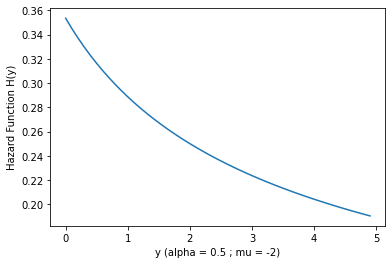
\includegraphics[width = \columnwidth]{solutions/2017/june/118/figures/Figure-1.png}
%     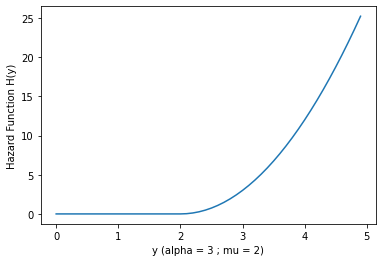
\includegraphics[width = \columnwidth]{solutions/2017/june/118/figures/Figure-2.png}
% \end{figure}
% \fi
\begin{figure}[h]
    \centering
    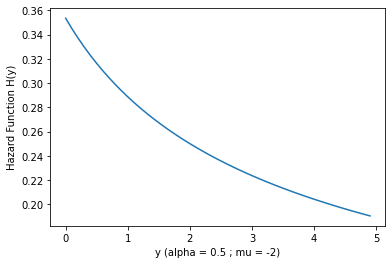
\includegraphics[width=\columnwidth-50pt]{solutions/2017/june/118/figures/Figure-1.png}
    \caption{Decreasing Hazard Function}
    \label{june/2017/118/fig:my_label1}
\end{figure}
\begin{figure}[h]
    \centering
    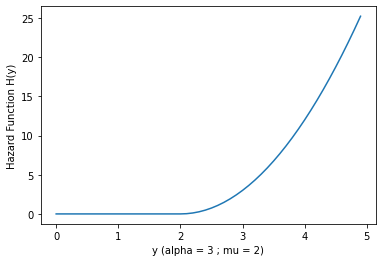
\includegraphics[width=\columnwidth-50pt]{solutions/2017/june/118/figures/Figure-2.png}
    \caption{Increasing Hazard Function}
    \label{june/2017/118/fig:my_label2}
\end{figure}


% \item $X_1$ and $X_2$ are independent Poisson variables such that $\pr{X_1=2} = \pr{X_1=1}$ and $\pr{X_2=2} = \pr{X_2=3}$. What is the variance of $(X_1 - 2X_2)$ ?
% \begin{enumerate}
%     \item 14
%     \item 4
%     \item 3
%     \item 2
% \end{enumerate}
% \solution
% For a Poisson variable X,
\begin{align}
\pr{X=k} = \frac{\lambda^{k}e^{-\lambda}}{k!}
\end{align}
Since $\pr{X_1=2} = \pr{X_1=1}$,
\begin{align}
\frac{{\lambda_1}^{2}e^{-{\lambda_1}}}{2!} &= \frac{{\lambda_1}^{1}e^{-{\lambda_1}}}{1!} \\
\lambda_1 &= 2!/1! = 2
\end{align}
Similarly, as $\pr{X_2=2} = \pr{X_2=3}$,
\begin{align}
\frac{{\lambda_2}^{2}e^{-{\lambda_2}}}{2!} &= \frac{{\lambda_2}^{3}e^{-{\lambda_2}}}{3!} \\
\lambda_2 &= 3!/2! = 3
\end{align}
Also we know for a Poisson variable X, the following holds true:
\begin{align}
\E[X] &= \lambda \\
\Var[X] &= \lambda \label{june/2017/108/eq1} \\
\Var[X] &= \E[X^2] - (\E[X])^2 \label{june/2017/108/eq2} 
\end{align}
Now, for the variance of $(X_1 - 2X_2)$
\begin{align}
\Var[X_1 - 2X_2] &= \E[(X_1 - 2X_2)^2] - (\E[X_1 - 2X_2])^2 \nonumber \\
&= \E[X_1^2 + 4X_2^2 - 4X_1X_2] \nonumber \\
&- (\E[X_1] - 2\E[X_2])^2 \nonumber \\
&= \E[X_1^2] - (\E[X_1])^2 + 4\E[X_2^2] \nonumber \\
& -4(\E[X_2])^2) + 4\E[X_1X_2] \nonumber \\
& + 4\E[X_1]\E[X_2]
\end{align}
Since the variables are independent:
\begin{align}
\E[X_1X_2] = \E[X_1]\E[X_2]
\end{align}
Substituting equations \eqref{june/2017/108/eq1} and \eqref{june/2017/108/eq2}, we get:
\begin{align}
\Var[X_1 - 2X_2] &= \Var[X_1] + 4(\Var[X_2]) \nonumber \\
&- 4\E[X_1][X_2] + 4\E[X_1][X_2] \nonumber \\
&= \lambda_1 + 4\lambda_2 = 2 + 4(3) = 14
\end{align}
Hence option (a) 14 is correct.
\end{enumerate}